\chapter{序論}

\section{研究背景}
近年なくしものの対策としてスマートタグという製品が普及している。
スマートタグとは貴重品などに取り付け, 紛失した際に捜索を補助するデバイスである. 
%@@@ 1: いきなり出てきてないものの説明をするよりは, 世の中にスマートタグというものがあってどういうふうに役に立っているかを先に説明する. @@@
補助の方法はタグが音を鳴らす方法と付近のスマートフォンと無線通信する方法が一般的である. 
しかし特性上タグの取り付けが困難な物もある. 
例えば入れ歯は口内で使用するために衛生や防水, 日常生活の邪魔になるなどの理由で取り付けが難しい. 

\section{関連研究}
タグを必要としないなくしもの対策として, 草野\index{くさの@草野}らが提案する家庭内での移動マニピュレータによるベイズ推定と自然言語処理を用いた物品捜索手法\cite{kusano}がある. 
%@@@↑タイトルをそのまま埋め込まない. ちゃんと言い換える@@@
この手法ではまず捜索範囲をいくつかのエリアに区切る. 
そして各エリアごとに過去そのエリアを捜索し捜索対象を発見した回数$\alpha$, 発見できなかった回数$\beta$を用い, 
捜索対象の存在確率を$ \alpha / (\alpha + \beta)$と定義し, 存在確率が最大のエリアを捜索する. 
また存在確率が最大のエリアが複数ある場合は
%@@@↑そうだったっけ?@@@
移動マニピュレータが位置するエリアからの距離, 
ならびに自然言語処理によるエリア内の家具の名前と捜索対象の名前の類似度も考慮する. 

\begin{figure}[H]
    \begin{center}
        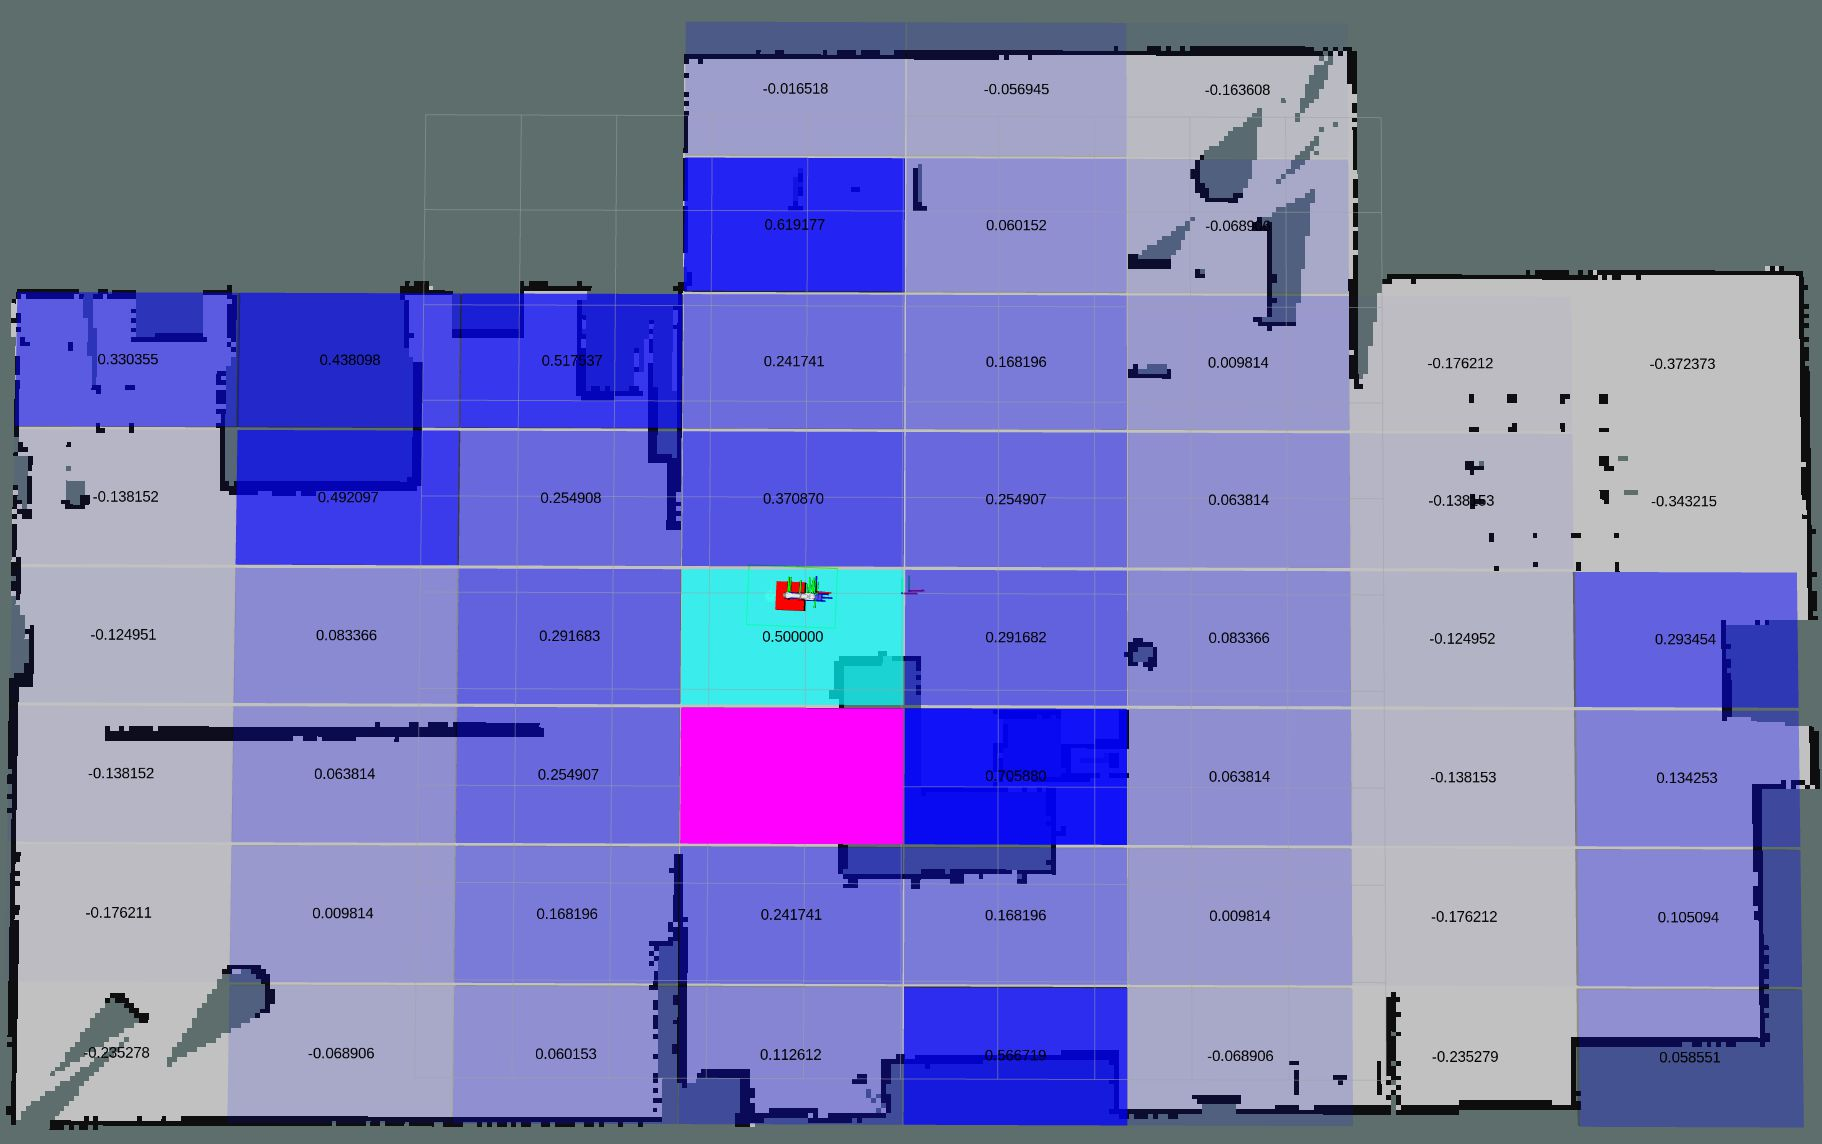
\includegraphics[width=0.8\linewidth]{figs/kusano.jpg}
        \caption{捜索対象の存在確率を表したヒートマップ\cite{kusano}}%@@@ 1: 出典書きましょう@@@
        \label{fig:kusano}
    \end{center}
\end{figure}

この手法は捜索する主体が移動マニピュレータであることを前提としている. 
なくしものの捜索はなくしものがある場所を予測する部分と予測した場所に移動し周辺を見回すという部分に分解できるが、
この手法では双方が密接に結びついているために移動マニピュレータが必要となる. 
しかし現在, そうしたロボットはスマートタグの代替としては高価であり利用できる環境は限定される. 

また, 人はなくしものを捜索する際に捜索対象物
%@@@ 1:「物」が抜けてる@@@
の所有者(以下, 単に所有者という)の行動を手がかりにする。
例えば所有者がよく使う場所を重点的に捜索する等である。
%@@@ 1: ↑主語がよくわからないです@@@
一方この手法の場合, なくしものは発生頻度が高くないため
$\alpha$が同じエリアが複数ある状況が長く続くことが想定される. 
%@@@ 1: ↑ここ, 舌足らずで伝わらんのでもうちょっと説明を足しましょう. あと主語を明確に. @@@
こうした状況ではエリア間の距離と単語の類似度を重視することになるが, これらは所有者の行動を反映していない. 

%@@@ 1: ↓の研究目的に書いてあるような議論は, 目的に入る前にここで節を設けて書きましょう. 目的に入る頃には何をするのか大体の人が予想できるようにする. @@@

\section{研究目的}
%@@@ 1: ↑これだと「考える」が目的になっちゃいます. @@@
本研究では移動等の部分は扱わず, なくしものの位置を推定する手法を提案する. 
位置推定にあたり所有者の行動を反映するため, なくしものが発生するまでの過程を確率論を用いてモデル化する. 
また提案手法の有効性を確認する準備として, なくしものの位置を推定するソフトウェアと推定に用いるパラメータの機械学習のためのシステムの開発も行う. 
